% \usetikzlibrary{calc,patterns,angles,quotes}

\begin{figure}[h]
    \centering
    
    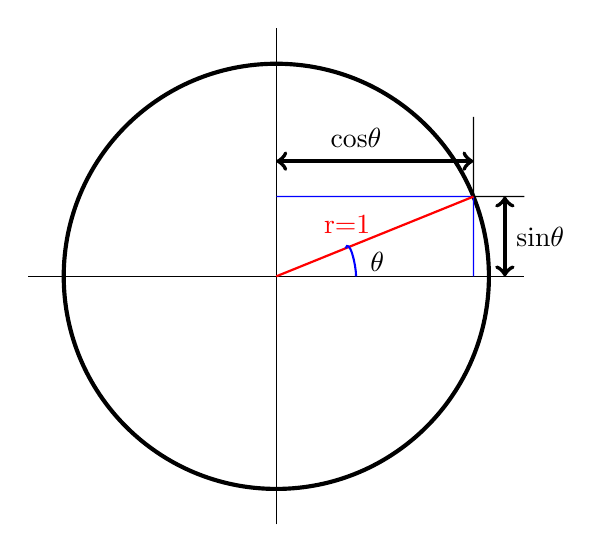
\begin{tikzpicture}[scale=0.45]
        \coordinate (center)  at (0,0);
        \coordinate (cuttoff) at (5.56215,2.25);

        % axes
        \draw [line width=.45pt] (-7,0) -- (7,0);
        \draw [line width=.45pt] (0,-7) -- (0,7);

        \draw [line width=1.5pt,circle] (center) circle [radius=6];
        
        %parallel to x axis
        \draw [blue,line width=.45pt] (0,2.25) -- (cuttoff);  
        \draw [black,line width=.45pt] (cuttoff) -- (7,2.25);

        %parallel to y axis
        \draw [blue,line width=.45pt] (5.56215,0) -- (cuttoff); 
        \draw [black,line width=.45pt] (cuttoff) -- (5.56215,4.5); 
        
        % rad line
        \draw [red,line width=.80pt] (center) -- (cuttoff); 
        \node [red,below] at (2,2) {r=1};
        
        % theta
        \draw [blue,line width=.75pt] (2.25,0) to [out=90,in=70] (1.95,0.7888136781);
        \node [above] at (2.85,-0.15) {$\theta$};
        % \pic [draw=blue, "$\theta$", angle eccentricity=1.5] {angle = (2.25,0)--(1.95,0.7888136781)};
        
        % sin
        \draw [<->=latex,line width=1.5pt] (6.45,0) -- (6.45,2.25);
        \node [right] at (6.5,1.125) {sin$\theta$};
        
        % cos
        \draw [<->=latex,line width=1.5pt] (0,3.25) -- (5.56215,3.25);
        \node [above] at (2.25,3.35) {cos$\theta$};
           
    \end{tikzpicture}
    
    \caption{Alternate representation of Pythagorean theorem.}
    \label{fig:fig2}
\end{figure}